% !TEX encoding = UTF-8 Unicode
\documentclass[a4paper]{article}
%\usepackage[T1]{fontenc}     % För svenska bokstäver
\usepackage[utf8]{inputenc}  % Teckenkodning UTF8
%\usepackage[swedish]{babel}  % För svensk avstavning och svenska
                            % rubriker (t ex Innehållsförteckning)
\usepackage{fancyvrb}        % För programlistor med tabulatorer
\fvset{tabsize=4}            % Tabulatorpositioner
\fvset{fontsize=\small}      % Lagom storlek för programlistor
\usepackage[labelfont=bf]{caption}
\usepackage{hyperref}
\usepackage{graphicx}         % För att inkludera bilder.
\usepackage{float}

\title{Lego Mindstorm Project: Lego Segway\\
FRTN01 - Real time systems}
\author{Simon Wallström, dat11swa@student.lu.se\\
Adam Dalentoft, dat11ada@student.lu.se\\
Jonathan Karlsson, ada09jka@student.lu.se\\\\
Supervisor: Victor Millnert}
%\date{1 augusti 1994}        % Blir dagens datum om det utelämnas
\begin{document}              % Början på dokumentet

\maketitle
\thispagestyle{empty}
\newpage
\setcounter{page}{1}
\tableofcontents
\newpage
\section{Introduction}
The goal of this project is to build and control a two-wheeled robot - a Lego Segway - using NXT Lego Mindstorm 2.0. A segway is an unstable system that constantly needs to be regulated to work. To regulate this system several parameters is required. It is important to know the mass and specifications of the hardware that is used and the physics and movements in the system. Basically how it works is that the the robot tilts and the angle is measured. Thereafter the angle is processed by the controller to calculate the required change power and direction of the motors. It is possible to control the segway in a few different ways. One way is to use pole placing and feedback control. Even though this is a good way to regulate the system it is not the first choice. Instead, the structure that will be described in this report uses two PID controllers, one for the wheel position and one for the angle of the robot. Later, the structure is changed to a state feedback controller due to lack of time, more about this later.

\begin{figure}[H]
 \centering
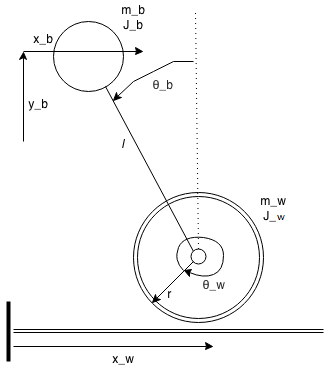
\includegraphics[scale=0.8]{pic/segway.png}
\caption{Model over the segway movements, all variables and their names are set in the picture. Values on the variables is given in the results.}
\end{figure}

Before the implementation can begin it is a good idea to set up a model of the process. The process is described in the picture, including the different variables that is needed to calculate the movements in the system. These variables are then used to calculate the state-space form for the system, describing the equation L = T - V. The state-space form of the system can thereafter be used in matlab and simulink to describe a control system for the segway. Simulink can also be used to make a simulation of the calculated system to determine parameters for the PID-controllers. \\

To implement the controller a Java version for Lego NXT is used called LeJOS. There are several alternatives in other languages but this is the only widely known Java VM. LeJOS provides classes for the most common hardware to the Lego NXT\cite{lejos}.  \\

To measure the angles a gyroscope and an accelerometer are used. The gyroscope measure the angle velocity and the integrated value gives the angle of the tilted segway. However the gyroscopes raw value drifts and therefore the accelerometer is required to compensate for this. Rest of the hardware is standard nxt motors and base unit.

\section{Program structure}
The program uses threads to realize a real time controlled system. The LeJOS VM provides support for real time threads and synchronization, the same as standard Java. There is a variety of classes building up the program, these are described in the diagram below. To clarify the meaning of the different classes there is also a brief description of them.

\begin{figure}[H]
 \centering
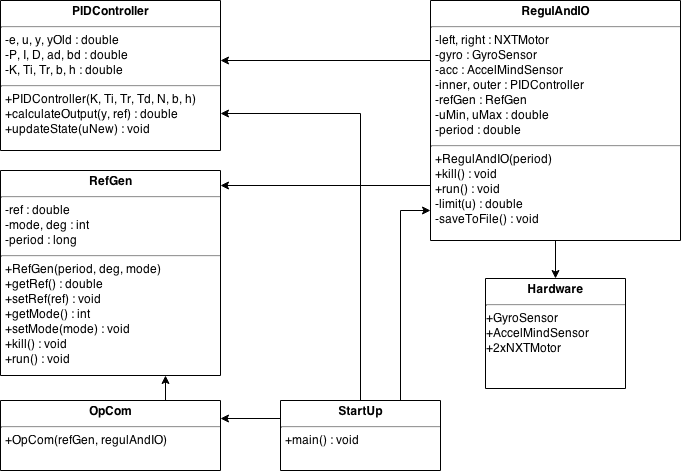
\includegraphics[scale=0.5]{pic/UML_LEGO_SEGWAY_ALLCAPS.png}
\caption{UML diagram of the classes for the PID controller.}
\end{figure}

\begin{itemize}
\item StartUp: main class, starts all the other classes and threads.
\item OpCom: Operator communication class, handles user input through passive listeners on the buttons on the base unit. Some of the commands are mode change and program exit.
\item RefGen: Reference generator. Generate reference values for input to the robot.
\item RegulAndIO: Control class and hardware communicator. Uses the PIDController class together with the hardware input and output to run and balance the segway.
\item PIDController: Controller class. Calculate the P, I and D values using a standard control equation from lecture 8\cite{L8}.
\item Hardware: All the hardware connected to the software together with their in and output methods.
\item FeedbackController: Controller class for the feedback controller. Not included in the original design and replaces RegulAndIO and PIDController. Otherwise it is connected in the same way as those classes.
\end{itemize}

\begin{figure}[H]
 \centering
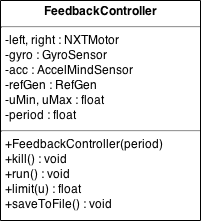
\includegraphics[scale=0.8]{pic/OnlyFeedback.png}
\caption{UML diagram of the Feedback class that is used instead of the RegulAndIO class.}
\end{figure}

\section{Control design}
As mentioned in the introduction the controller will contain two PID-controllers. They are connected in a cascade to regulate the two angles: tilt angle and wheel angle (rotation of the wheel). The inner loop controls the tilt angle by moving the wheels and the outer loop controls the wheel position in case of a reference change and to make sure the robot doesn't drift when standing still.

\begin{figure}[H]
  \centering
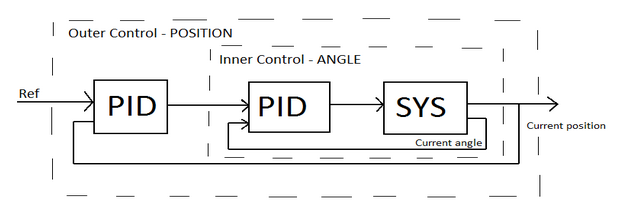
\includegraphics[scale=0.8]{pic/PIDs.png}
\caption{Figure over the PID controllers. The inner loop controls the angle of the segway and the outer the position of the wheels.}
\end{figure}

The main reason for this choice of control structure is the rather easy way to implement it. As mentioned in the introduction there are other ways to control the system, but this method has been used earlier in the course which made it the first choice and more natural to implement. \\

The figure describes how the control structure works. First the reference value is sent in. It can either be 0, to stand still, or a value decided by the reference generator. The mode is decided by the user (further description in the user information section). This value describes the desired position of the segway. Thereafter the value, together with the feedback values from the previous calculations, is processed by the two PID-controllers. When the segway should stand still only the inner loop is required. \\

An optional solution is to use state feedback. Here the different measurements (angle, position, angular velocity and wheel movement) of the system is fed back and thereby the different states of the system is regulated based on previous location and value. This version got a structure like the second figure in this section. The phi value controls the angle of the robot, phi dot the angular velocity, theta the wheel movement and theta dot the wheel velocity. \\

\begin{figure}[H]
 \centering
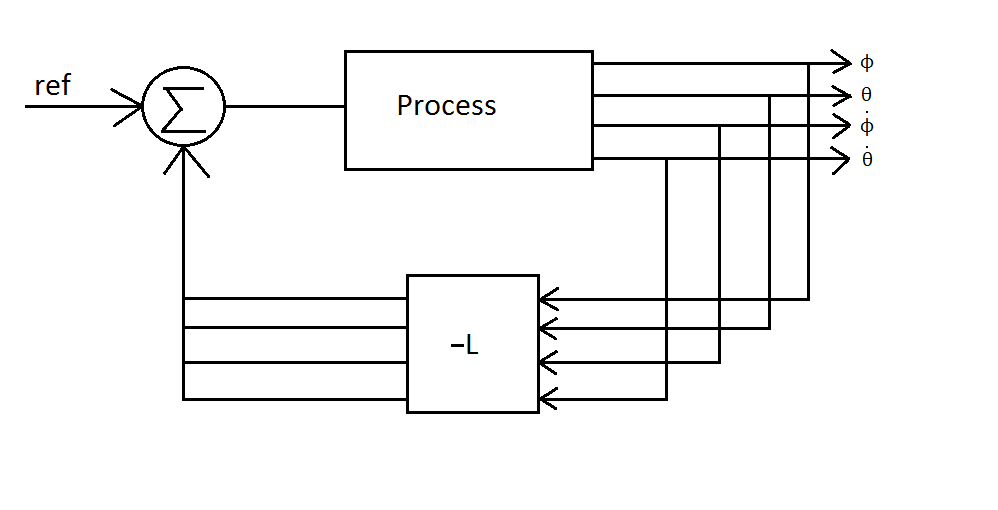
\includegraphics[scale=0.5]{pic/Statefeedback.png}
\caption{Figure over the control scheme of the state feedback version of the controller.}
\end{figure}

\section{User information}

The segway do not have a user interface except the small screen and the buttons on the front of the base unit. When the segway is in motion these become a rather impractical way of controlling the system. Therefore the system is started before it is put down. It is however possible to change mode with the buttons from stand still mode and a mode that changes the reference value to make the robot move forward and backward. A press on the dark grey button, the Escape button, will quit the program. The screen give out small messages to inform the user how to handle the robot and what is happening in the system.\\

The program should be pre-installed on the machine. To run it is done in a few simple steps.

\begin{enumerate}
\item First start the segway using the large yellow button, the Enter button.
\item On the screen a menu will be displayed. Choose the default program on the screen.
\item Now the program starts. A message will be displayed, “Calibrating...”. It is important to hold the robot stationary, otherwise the calibration of the hardware may be disturbed.
\item After the calibration, the message "Calibrated, hold robot and press Enter to balance" is shown. Now, put down the robot on the ground and press the Enter key.
\item After the massage “Balancing” is displayed the segway will start to balance, hopefully.
\item If a different mode than the default one is selected the balancing point may differ and the segway will move forward and backward.
\item To terminate the program push the Escape key.
\end{enumerate}

\section{Results}
\subsection{Parameters and values}
\subsubsection*{Model values}
$J_w = 1.6*10^-5$ Wheel inertia \\
$R_w = 0.08$ Wheel radius \\
$L = 0.0950$ Length from wheel to body mass \\
$m_b = 0.5120$ Body mass \\
$m_w = 0.031$ Combined mass of both wheels \\
$J_b = 0.0019$ Body inertia \\
$b = 0.062$ Damping factor \\
$g = 9.81$ Gravity \\ \\

\subsubsection*{L values}
$L_1=-23.8$\\
$L_2=0$\\
$L_3=-0.155$\\
$L_4=0$\\ \\

\subsubsection*{PID values (approximate, do not work)}
$K=9$\\
$Ti=2$\\
$Tr=1$\\
$Td=0.1$\\
$N=10$\\ \\

\subsubsection*{Filter equations}
Complementary: $GyroAngle * 0.98 + AccelerometerAngle*0.02$ \\
Low pass: $G_{lp} = \frac{1}{s+1}$\\
High pass: $G_{hp} = \frac{s}{s+10}$\\

\subsection{Hardware}

\begin{figure}[H]
 \centering
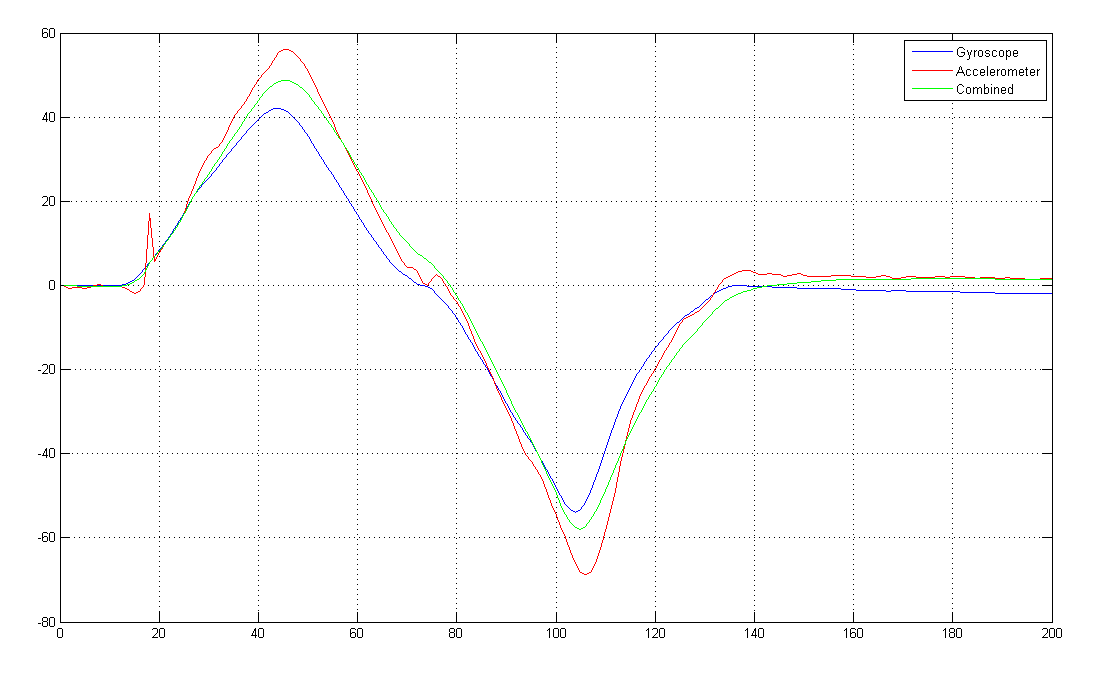
\includegraphics[scale=0.4]{pic/GyroAccCombAng.png}
\caption{The figure describes the relation between the gyroscope and the accelerometer, together with the complementary filter.}
\end{figure}

\begin{figure}[H]
  \centering
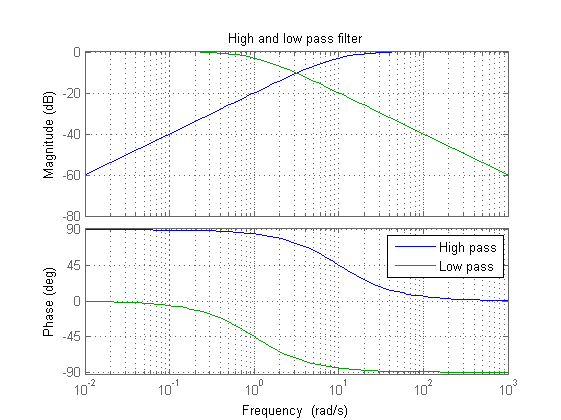
\includegraphics[scale=0.8]{pic/HP_LP.png}
\caption{High and low pass filter used to filter signals from gyroscope respectively accelerometer.}
\end{figure}

%Lägg in ny bild med värden från hög och lågpass filtrerna.

\subsection{PID Controller}
\begin{figure}[H]
  \centering
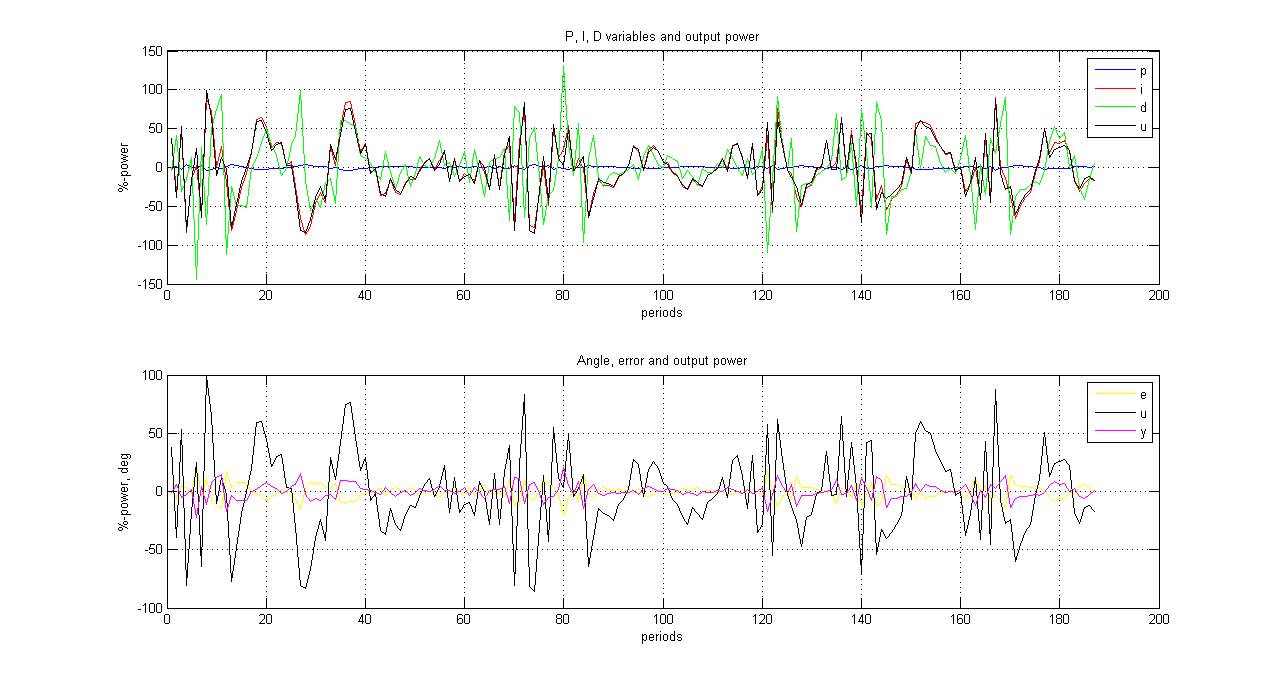
\includegraphics[scale=0.45]{pic/pid.png}
\caption{Relation between the different parameters in the PID controller.}
\end{figure}

\subsection{Feedback Controller}
\begin{figure}[H]
  \centering
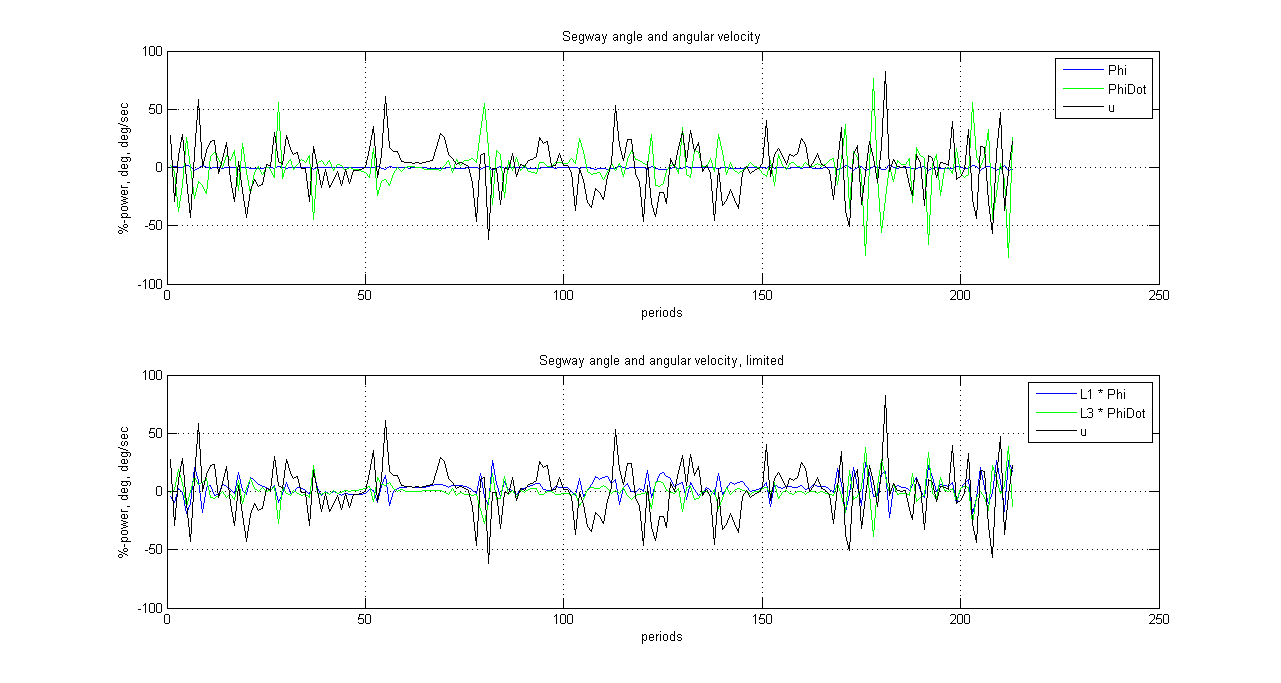
\includegraphics[scale=0.45]{pic/feedbackPlot.png}
\caption{Relation between the different parameters in the feedback controller for the angle of the segway.}
\end{figure}

\section{Conclusion}
The project in itself is a good example of real-time-programming and control. To complete the project it is required to have knowledge in both of the areas. Even though implementing a segway is a common control task (both as a Lego mindstorms project and other) is it not an easy task. There are numerous of factors that can go wrong.\\

As for all realizations of theory there are error sources, this is no exception. To start with, the hardware is not perfect. As previously mentioned the gyroscope drifts, that is because of temperature shifts, among other things. This was originally solved by using the gyroscope and an accelerometer in a complementary filter to smooth out the measurements and thereby eliminate the drift. The final solution is to filter the gyroscope value in a high pass filter to get rid of the drift over time and add a low pass filtered accelerometer value to get rid of the flickering in sudden changes. Even though the gyroscope problem is solved the accelerometer introduce another problem by adding a couple of milliseconds to the control loop. Thereby the period has to be increased which makes the whole system slower and harder to control. The rest of the hardware can also give errors, such as the motors being unsynchronized, cable problems and computing errors in the base unit\cite{filter}.\\

The software implementation can also give some errors, especially the parameters of the controllers. Tuning the parameters is extremely time consuming and even the smallest change can give a large difference.\\

Because of the many error sources the optional solution may give a more stable control. The new solution is the one previously discussed, a feedback loop where the different states of the segway is used to control the movements. This other solution is easier to tune and therefore less time has to be spent, especially good when time is of the essence. In terms of control, there is no considerable difference. To compare the plots from the two is a bit hard as well because of the different parameters used when controlling. However, because of the differences this gives a good indication on how systems can be controlled in many different ways with the same results, it all comes down to preferences. \\

Because of the many problems and the change of controller the result of the project was not the expected one. Many changes had to be made along the way to try fix the errors constantly occurring. The implementation had different stages where different combinations of threads and monitors were used, mostly because of optimization to fit the real time requirements. The most time consuming part of the project was tuning the PID parameters, this part felt very tiresome and much work made little progress. Because of this the decision to change the control design to a state-space feedback was considered, because the segway had problems stabilising with the PID controller. This new method was rather new and unexplored because all the preparations and simulations were made matching the first solution. Things that could have been made different is things like research on different controllers before the implementation and take more basic things in consideration like hardware problems.

\section{Acknowledgements}

\begin{thebibliography}{1}
\bibitem{lejos}
LEJOS NXT, Java for LEGO Mindstorms\\
\url{http://www.lejos.org/nxj.php}\\
(Hämtad 14/12-14)

\bibitem{L8}
Lecture 8, Real-Time Systems LTH, 23/9-14\\
\url{http://www.control.lth.se/media/Education/EngineeringProgram/FRTN01/2014/L8_14.pdf}\\
(Hämtad 14/12-14)

\bibitem{filter}
The Balance Filter, Shane Colton, 25/6-07\\
\url{https://b94be14129454da9cf7f056f5f8b89a9b17da0be.googledrive.com/host/0B0ZbiLZrqVa6Y2d3UjFVWDhNZms/filter.pdf}\\
(Hämtad 10/12-14)
\end{thebibliography}

\end{document}                  % Slut på dokumentet



%\begin{figure}[H]
%  \centering
%\includegraphics[scale=0.8]{xXx.png}
%\caption{el caprioneE}
%\end{figure}

